\documentclass[12pt,a4paper]{article}
\usepackage[utf8]{vietnam}
\usepackage{amsmath,amssymb}
\usepackage{geometry}
\geometry{top=1.5cm,bottom=1.2cm,left=1.4cm,right=1.4cm,headheight=28pt,headsep=12pt,footskip=18pt}
\usepackage{tikz}
\usepackage{xcolor}
\usepackage{enumerate}
\usepackage{graphicx}
\usepackage[version=4]{mhchem}
\usepackage{fancyhdr}
\usepackage{ex_test}

\renewcommand{\baselinestretch}{0.96}
\setlength{\parskip}{0pt}

\definecolor{hfRed}{RGB}{211,47,47}
\definecolor{hfGreen}{RGB}{139,195,144}

\pagestyle{fancy}
\fancyhf{}
\fancyhead[L]{\small\itshape\color{hfRed} Tài liệu lưu hành nội bộ}
\fancyhead[R]{\small\itshape\color{hfRed} Thầy \textbf{TRẦN VĂN THẠNH} - 0777.470.803}
\renewcommand{\headrulewidth}{0.8pt}
\renewcommand{\headrule}{\hbox to\headwidth{\color{hfGreen}\leaders\hrule height \headrulewidth\hfill}}

\fancyfoot[L]{\small\itshape\color{hfRed} CS1: 6/15 Nguyễn Hoàng, P. Kim Long, TP Huế \quad|\quad CS2: 24 Đặng Thái Thân, TP Huế}
\fancyfoot[R]{\small\bfseries\color{hfRed} Trang \thepage}
\renewcommand{\footrulewidth}{0.8pt}
\renewcommand{\footrule}{\hbox to\headwidth{\color{hfGreen}\leaders\hrule height \footrulewidth\hfill}}

\fancypagestyle{firstpage}{
  \fancyhf{}
  \renewcommand{\headrulewidth}{0pt}
  \fancyfoot[L]{\small\itshape\color{hfRed} CS1: 6/15 Nguyễn Hoàng, P. Kim Long, TP Huế \quad|\quad CS2: 24 Đặng Thái Thân, TP Huế}
  \fancyfoot[R]{\small\bfseries\color{hfRed} Trang \thepage}
  \renewcommand{\footrulewidth}{0.8pt}
  \renewcommand{\footrule}{\hbox to\headwidth{\color{hfGreen}\leaders\hrule height \footrulewidth\hfill}}
}

\begin{document}
\thispagestyle{firstpage}

\noindent
\begin{minipage}[t]{0.44\textwidth}
	\centering\fontsize{10pt}{12pt}\selectfont
	\textbf{SỞ GIÁO DỤC VÀ ĐÀO TẠO THỪA THIÊN HUẾ}\\
	\textbf{ĐỀ CHÍNH THỨC}\\
	\textit{(Đề thi có 04 trang)}
\end{minipage}\hfill
\begin{minipage}[t]{0.54\textwidth}
	\centering\small
	\textbf{ĐỀ KIỂM TRA ĐỊNH KỲ CHƯƠNG 1 (CÂN BẰNG HÓA HỌC)}\\
	\textbf{MÔN: HOÁ HỌC -- LỚP 11}\\
	\textit{Thời gian làm bài: 45 phút (không kể thời gian phát đề)}\\
	\fbox{\textbf{MÃ ĐỀ: 101}}
\end{minipage}

\smallskip
\begin{center}
	{\color{hfRed}\textbf{\large (BẢN GIÁO VIÊN -- CÓ LỜI GIẢI CHI TIẾT)}}
\end{center}

\smallskip
\noindent\hrulefill
\smallskip

\noindent\textbf{Họ, tên thí sinh:} \dotfill\ \textbf{Lớp:} \dotfill\ \textbf{Số báo danh:} \dotfill

\smallskip
\noindent\textit{(Cho biết nguyên tử khối: H = 1; C = 12; N = 14; O = 16; Na = 23; Al = 27; S = 32; Cl = 35,5; K = 39; Ca = 40; Ba = 137).}
\smallskip

\noindent
\textbf{PHẦN I (4,5 điểm -- 18 câu): Câu trắc nghiệm nhiều phương án lựa chọn.}\\
\textit{Thí sinh trả lời từ câu 1 đến câu 18. Mỗi câu hỏi thí sinh chỉ chọn một phương án.}

\Opensolutionfile{ans}[ans-hoa11-de01gv]

\begin{ex}
Trong cùng điều kiện xác định, kết luận nào sau phản ứng xảy ra từ chất tham gia tạo thành chất sản phẩm. Kết luận nào sau đây là đúng?
\choice
{Nếu chất sản phẩm không thể tác dụng với nhau để tạo lại chất ban đầu thì đó là phản ứng thuận nghịch.}
{Nếu chất sản phẩm có thể tác dụng với nhau để tạo lại chất ban đầu thì đó là phản ứng một chiều.}
{Nếu chất sản phẩm có thể tác dụng với nhau để tạo lại chất khác thì đó là phản ứng thuận nghịch.}
{\True Nếu chất sản phẩm có thể tác dụng với nhau để tạo lại chất ban đầu thì đó là phản ứng thuận nghịch.}
\loigiai{
Phản ứng thuận nghịch là phản ứng trong cùng điều kiện xác định, chất phản ứng tạo thành chất sản phẩm và các chất sản phẩm cũng có thể tác dụng với nhau để tạo lại chất phản ứng ban đầu.\\
\textbf{Chọn D.}}
\end{ex}

\begin{ex}
Trong phản ứng thuận nghịch, kết luận nào sau đây là đúng tại thời điểm ban đầu?
\choice
{Tốc độ phản ứng thuận bằng tốc độ phản ứng nghịch.}
{Nồng độ các chất trong hệ phản ứng không đổi.}
{Tốc độ phản ứng nghịch bằng 0 sau đó giảm dần.}
{\True Tốc độ phản ứng thuận đạt lớn nhất sau đó giảm dần.}
\loigiai{
Tại thời điểm ban đầu, nồng độ các chất phản ứng lớn nhất nên tốc độ phản ứng thuận lớn nhất, sau đó giảm dần theo thời gian. Nồng độ chất sản phẩm bằng 0 nên tốc độ phản ứng nghịch bằng 0, sau đó tăng dần.\\
\textbf{Chọn D.}}
\end{ex}

\begin{ex}
(SGK - CD): Phát biểu nào sau đây về một phản ứng thuận nghịch tại trạng thái cân bằng là sai?
\choice
{Tốc độ của phản ứng thuận bằng tốc độ của phản ứng nghịch.}
{Nồng độ của tất cả các chất trong hỗn hợp phản ứng là không đổi.}
{\True Nồng độ mol của chất phản ứng luôn bằng nồng độ mol của chất sản phẩm phản ứng.}
{Phản ứng thuận và phản ứng nghịch vẫn diễn ra.}
\loigiai{
Tại trạng thái cân bằng, tốc độ phản ứng thuận bằng tốc độ phản ứng nghịch và nồng độ của các chất không thay đổi theo thời gian, nhưng không nhất thiết nồng độ chất phản ứng phải bằng nồng độ chất sản phẩm.\\
\textbf{Chọn C.}}
\end{ex}

\begin{ex}
Phản ứng nào sau đây là phản ứng thuận nghịch?
\choice
{$\ce{Mg + 2HCl -> MgCl2 + H2}$.}
{\True $\ce{H2 + I2 <=> 2HI}$.}
{$\ce{C2H5OH + 3O2 ->[t^\circ] 2CO2 + 3H2O}$.}
{$\ce{2KClO3 ->[t^\circ] 2KCl + 3O2}$.}
\loigiai{
Phản ứng $\ce{H2(g) + I2(g) <=> 2HI(g)}$ là phản ứng thuận nghịch điển hình. Các phản ứng còn lại là phản ứng một chiều.\\
\textbf{Chọn B.}}
\end{ex}

\begin{ex}
Trong số các dung dịch có cùng nồng độ mol sau đây, dung dịch nào có độ dẫn điện yếu nhất?
\choice
{$\ce{NaCl}$}
{$\ce{CH3COONa}$}
{\True $\ce{CH3COOH}$}
{$\ce{H2SO4}$}
\loigiai{
$\ce{NaCl}, \ce{CH3COONa}$ là các chất điện li mạnh (muối tan hoàn toàn thành ion). $\ce{H2SO4}$ là acid mạnh điện li mạnh. $\ce{CH3COOH}$ là acid yếu, chất điện li yếu (chỉ phân li một phần nhỏ thành ion) nên có nồng độ ion tự do nhỏ nhất ➔ dẫn điện yếu nhất.\\
\textbf{Chọn C.}}
\end{ex}

\begin{ex}
Cho các chất dưới đây: $\ce{HClO4}, \ce{HClO}, \ce{HF}, \ce{HNO3}, \ce{H2S}, \ce{H2SO3}, \ce{NaOH}, \ce{NaCl}, \ce{CuSO4}, \ce{CH3COOH}$. Số chất thuộc loại chất điện li mạnh là
\choice
{\True 5.}
{6.}
{7.}
{4.}
\loigiai{
Các chất điện li mạnh gồm: acid mạnh ($\ce{HClO4}, \ce{HNO3}$), base mạnh ($\ce{NaOH}$), muối tan ($\ce{NaCl}, \ce{CuSO4}$) ➔ Tổng cộng có 5 chất. Các chất còn lại ($\ce{HClO}, \ce{HF}, \ce{H2S}, \ce{H2SO3}, \ce{CH3COOH}$) là chất điện li yếu.\\
\textbf{Chọn A.}}
\end{ex}

\begin{ex}
Trong dung dịch loãng của các chất khác nhau, tích số ion của nước chỉ phụ thuộc vào yếu tố nào sau đây?
\choice
{nồng độ}
{thể tích}
{\True nhiệt độ}
{áp suất}
\loigiai{
Tích số ion của nước $K_w = [\ce{H+}][\ce{OH-}]$ là một hằng số cân bằng, do đó nó chỉ phụ thuộc vào nhiệt độ. Ở $25^\circ\text{C}$, $K_w = 1,0 \cdot 10^{-14}$.\\
\textbf{Chọn C.}}
\end{ex}

\begin{ex}
Dung dịch nào dưới đây dẫn điện tốt nhất?
\choice
{$\ce{NaI}\ 0{,}002\text{M}$}
{$\ce{NaI}\ 0{,}010\text{M}$}
{\True $\ce{NaI}\ 0{,}100\text{M}$}
{$\ce{NaI}\ 0{,}001\text{M}$}
\loigiai{
$\ce{NaI}$ là chất điện li mạnh. Cùng một chất điện li mạnh thì dung dịch có nồng độ càng lớn sẽ có mật độ ion tự do càng cao, do đó dẫn điện càng tốt ➔ $\ce{NaI}\ 0{,}100\text{M}$ dẫn điện tốt nhất.\\
\textbf{Chọn C.}}
\end{ex}

\begin{ex}
{[CD - SBT]} Đối với phản ứng sau, cân bằng sẽ bị ảnh hưởng như thế nào khi tăng nhiệt độ (các điều kiện khác giữ không đổi)?
\[ \ce{H2(g) + 1/2 O2(g) <=> H2O(l)} \quad \Delta_r\text{H}^\circ_{298} = -296\text{ kJ} \]
\choice
{Cân bằng chuyển dịch sang phải.}
{\True Cân bằng chuyển dịch sang trái.}
{Không thay đổi.}
{Không dự đoán được sự chuyển dịch cân bằng.}
\loigiai{
$\Delta_r\text{H}^\circ_{298} = -296\text{ kJ} < 0 \implies$ phản ứng thuận toả nhiệt. Theo nguyên lí Le Chatelier, khi tăng nhiệt độ, cân bằng chuyển dịch theo chiều phản ứng thu nhiệt (chiều nghịch, tức là sang trái).\\
\textbf{Chọn B.}}
\end{ex}

\begin{ex}
{[CD - SBT]} Trong phản ứng nào sau đây sự tăng áp suất sẽ dẫn tới cân bằng chuyển dịch sang trái (các điều kiện khác coi như không thay đổi)?
\choice
{\True $\ce{CaCO3(s) <=> CaO(s) + CO2(g)}$}
{$\ce{CO(g) + H2O(g) <=> H2(g) + CO2(g)}$}
{$\ce{2H2(g) + O2(g) <=> 2H2O(l)}$}
{$\ce{C(s) + O2(g) <=> CO2(g)}$}
\loigiai{
Khi tăng áp suất, cân bằng chuyển dịch theo chiều làm giảm số mol khí.\\
- Phản ứng A: vế trái có 0 mol khí, vế phải có 1 mol khí $\ce{CO2}$. Chiều nghịch (sang trái) là chiều giảm số mol khí (từ 1 xuống 0) ➔ cân bằng chuyển dịch sang trái.\\
- B và D có số mol khí ở 2 vế bằng nhau (áp suất không ảnh hưởng).\\
- C có 3 mol khí vế trái và 0 mol khí vế phải (tăng áp suất chuyển dịch sang phải).\\
\textbf{Chọn A.}}
\end{ex}

\begin{ex}
Cho cân bằng hóa học: $\ce{CaCO3(rắn) <=> CaO(rắn) + CO2(khí)}$. Biết phản ứng thuận là phản ứng thu nhiệt. Tác động nào sau đây vào hệ cân bằng để cân bằng đã cho chuyển dịch theo chiều thuận?
\choice
{Giảm nhiệt độ.}
{Tăng áp suất.}
{Tăng nồng độ khí $\ce{CO2}$.}
{\True Tăng nhiệt độ.}
\loigiai{
Phản ứng thuận thu nhiệt ($\Delta_r\text{H} > 0$). Theo nguyên lí Le Chatelier, khi tăng nhiệt độ cân bằng sẽ chuyển dịch theo chiều thu nhiệt, tức là chiều thuận.\\
\textbf{Chọn D.}}
\end{ex}

\begin{ex}
Cho cân bằng hóa học: $\ce{PCl5(k) <=> PCl3(k) + Cl2(k)};\ \Delta_r\text{H}^\circ_{298} > 0$. Cân bằng chuyển dịch theo chiều thuận khi
\choice
{Thêm $\ce{PCl3}$ vào hệ phản ứng.}
{Tăng áp suất của hệ phản ứng.}
{\True Tăng nhiệt độ của hệ phản ứng.}
{Thêm $\ce{Cl2}$ vào hệ phản ứng.}
\loigiai{
$\Delta_r\text{H}^\circ_{298} > 0 \implies$ phản ứng thuận thu nhiệt. Khi tăng nhiệt độ, cân bằng chuyển dịch theo chiều thu nhiệt, tức chiều thuận.\\
\textbf{Chọn C.}}
\end{ex}

\begin{ex}
Cho các cân bằng sau:\\
(1) $\ce{2SO2(g) + O2(g) <=> 2SO3(g)}$\\
(2) $\ce{N2(g) + 3H2(g) <=> 2NH3(g)}$\\
(3) $\ce{CO2(g) + H2(g) <=> CO(g) + H2O(g)}$\\
(4) $\ce{2HI(g) <=> H2(g) + I2(g)}$\\
Khi thay đổi áp suất, nhóm gồm các cân bằng hoá học đều không bị chuyển dịch là
\choice
{(1) và (2).}
{(1) và (3).}
{\True (3) và (4).}
{(2) và (4).}
\loigiai{
Áp suất không làm chuyển dịch cân bằng của các phản ứng có tổng hệ số mol chất khí ở hai vế bằng nhau.\\
- Cân bằng (3): $1 + 1 = 1 + 1 = 2$ mol khí.\\
- Cân bằng (4): $2 = 1 + 1 = 2$ mol khí.\\
Vậy nhóm (3) và (4) không bị chuyển dịch khi thay đổi áp suất.\\
\textbf{Chọn C.}}
\end{ex}

\begin{ex}
Cho cân bằng hoá học: $\ce{N2(g) + 3H2(g) <=> 2NH3(g)}$; phản ứng thuận là phản ứng tỏa nhiệt. Cân bằng hoá học không bị chuyển dịch khi
\choice
{Thay đổi nồng độ $\ce{N2}$}
{\True Thêm chất xúc tác Fe.}
{Thay đổi nhiệt độ.}
{Thay đổi áp suất của hệ.}
\loigiai{
Chất xúc tác làm tăng tốc độ phản ứng thuận và nghịch với mức độ như nhau, giúp hệ nhanh đạt tới trạng thái cân bằng chứ không làm chuyển dịch cân bằng hoá học.\\
\textbf{Chọn B.}}
\end{ex}

\begin{ex}
(SGK-KNTT-Tr21): pH của dung dịch nào sau đây có giá trị nhỏ nhất?
\choice
{\True Dung dịch $\ce{HCl}\ 0{,}1\text{ M}$.}
{Dung dịch $\ce{CH3COOH}\ 0{,}1\text{ M}$.}
{Dung dịch $\ce{NaCl}\ 0{,}1\text{ M}$.}
{Dung dịch $\ce{NaOH}\ 0{,}01\text{ M}$.}
\loigiai{
Dung dịch acid có $\text{pH} < 7$, acid càng mạnh thì pH càng nhỏ.\\
- $\ce{HCl}$ là acid mạnh phân li hoàn toàn: $[\ce{H+}] = 0{,}1\text{ M} \implies \text{pH} = 1$.\\
- $\ce{CH3COOH}$ là acid yếu phân li một phần: $[\ce{H+}] < 0{,}1\text{ M} \implies \text{pH} > 1$.\\
- $\ce{NaCl}$ trung tính có $\text{pH} = 7$; $\ce{NaOH}$ có $\text{pH} = 12$.\\
Vậy $\ce{HCl}\ 0{,}1\text{ M}$ có pH nhỏ nhất.\\
\textbf{Chọn A.}}
\end{ex}

\begin{ex}
(SGK-KNTT-Tr22): Đo pH của một cốc nước chanh được giá trị pH bằng 2,4. Nhận định nào sau đây không đúng?
\choice
{Nước chanh có môi trường acid.}
{Nồng độ ion $[\ce{H+}]$ của nước chanh là $10^{-2{,}4}\text{ mol/L}$.}
{\True Nồng độ ion $[\ce{H+}]$ của nước chanh là $0{,}24\text{ mol/L}$.}
{Nồng độ của ion $[\ce{OH-}]$ của nước chanh nhỏ hơn $10^{-7}\text{ mol/L}$.}
\loigiai{
- A đúng vì $\text{pH} = 2{,}4 < 7 \implies$ môi trường acid.\\
- B đúng vì $[\ce{H+}] = 10^{-\text{pH}} = 10^{-2{,}4}\text{ mol/L}$.\\
- C sai vì $[\ce{H+}] = 10^{-2{,}4}\text{ mol/L} \approx 3{,}98 \cdot 10^{-3}\text{ mol/L} \neq 0{,}24\text{ mol/L}$.\\
- D đúng vì $[\ce{OH-}] = \frac{10^{-14}}{10^{-2{,}4}} = 10^{-11{,}6} < 10^{-7}\text{ mol/L}$.\\
\textbf{Chọn C.}}
\end{ex}

\begin{ex}
Cho các phát biểu sau:\\
(1) Khi phản ứng thuận nghịch đạt trạng thái cân bằng hóa học, phản ứng dừng lại.\\
(2) Cân bằng hóa học là cân bằng động.\\
(3) Khi thay đổi trạng thái cân bằng của phản ứng thuận nghịch, cân bằng sẽ chuyển dịch về phía chống lại sự thay đổi đó.\\
(4) Các yếu tố luôn ảnh hưởng đến cân bằng hoá học là: Nhiệt độ, nồng độ, áp suất.\\
(5) Phản ứng thuận nghịch là phản ứng xảy ra theo 2 chiều ngược nhau trong cùng một điều kiện.\\
(6) Phản ứng bất thuận nghịch là phản ứng xảy ra theo 1 chiều xác định.\\
(7) Cân bằng hóa học là trạng thái mà phản ứng đã xảy ra hoàn toàn.\\
(8) Khi phản ứng thuận nghịch đạt trạng thái cân bằng hóa học, lượng các chất sẽ không đổi.\\
Số phát biểu đúng là
\choice
{7}
{8}
{6}
{\True 5}
\loigiai{
Có 5 phát biểu đúng: (2), (3), (5), (6), (8).\\
- (1) Sai vì phản ứng vẫn diễn ra ở mức độ vi mô với tốc độ thuận bằng tốc độ nghịch.\\
- (4) Sai vì áp suất chỉ ảnh hưởng khi phản ứng có chất khí và có biến thiên số mol khí.\\
- (7) Sai vì phản ứng thuận nghịch không xảy ra hoàn toàn.\\
\textbf{Chọn D.}}
\end{ex}

\begin{ex}
{[CD - SBT]}
\begin{enumerate}[a)]
	\item Cốc A chứa 50 ml dung dịch $\ce{KOH}\ 0{,}10\text{M}$ được chuẩn độ với dung dịch $\ce{HNO3}\ 0{,}10\text{M}$. Sau khi thêm 52 ml dung dịch $\ce{HNO3}$ vào, pH của dung dịch trong cốc A là
	\choice
	{$2{,}80$.}
	{\True $2{,}71$.}
	{$2{,}40$.}
	{$3{,}00$.}
	\item Chuẩn độ 100,0 ml dung dịch $\ce{NaOH}\ 0{,}1\text{M}$ bằng dung dịch $\ce{HCl}\ 1{,}0\text{ M}$. Thể tích dung dịch $\ce{HCl}$ cần thêm để dung dịch thu được có $\text{pH} = 12$ là
	\choice
	{\True $8{,}91\text{ ml}$.}
	{$8{,}52\text{ ml}$.}
	{$9{,}01\text{ ml}$.}
	{$8{,}72\text{ ml}$.}
\end{enumerate}
\loigiai{
a) $n_{\ce{KOH}} = 0{,}050 \times 0{,}10 = 0{,}0050\text{ mol}$; $n_{\ce{HNO3}} = 0{,}052 \times 0{,}10 = 0{,}0052\text{ mol}$.\\
$\ce{H+ + OH- -> H2O} \implies n_{\ce{H+ dư}} = 0{,}0052 - 0{,}0050 = 0{,}0002\text{ mol}$.\\
$V_{\text{dd}} = 50 + 52 = 102\text{ mL} = 0{,}102\text{ L}$.\\
$[\ce{H+}] = \frac{0{,}0002}{0{,}102} \approx 1{,}961 \cdot 10^{-3}\text{ M} \implies \text{pH} = -\log(1{,}961 \cdot 10^{-3}) \approx 2{,}71$.\\
b) $n_{\ce{NaOH ban đầu}} = 0{,}100 \times 0{,}1 = 0{,}01\text{ mol}$. Gọi thể tích dung dịch $\ce{HCl}$ là $V\text{ (L)}$.\\
$\text{pH} = 12 \implies \text{pOH} = 2 \implies [\ce{OH-}] = 0{,}01\text{ M}$.\\
$[\ce{OH-}] = \frac{0{,}01 - V}{0{,}1 + V} = 0{,}01 \implies 0{,}01 - V = 0{,}001 + 0{,}01V \implies 1{,}01V = 0{,}009 \implies V \approx 8{,}91\text{ mL}$.\\
\textbf{Chọn a) B và b) A.}}
\end{ex}

\Closesolutionfile{ans}

\bigskip
\noindent
\textbf{PHẦN II (4,0 điểm -- 4 câu): Câu trắc nghiệm đúng sai.}\\
\textit{Thí sinh trả lời từ câu 1 đến câu 4. Trong mỗi ý a), b), c), d) ở mỗi câu, thí sinh chọn đúng hoặc sai.}

\begin{ex}
Trong bình kín có hệ cân bằng hóa học sau: $\ce{CO(g) + H2O(g) <=> CO2(g) + H2(g)};\ \Delta_r\text{H}^\circ_{298} > 0$.
\choiceTF
{\True a) Thêm một lượng hơi nước cân bằng chuyển dịch theo chiều thuận.}
{b) Thêm một lượng $\ce{CO2}$ cân bằng chuyển dịch theo chiều thuận.}
{c) Giảm áp suất chung của hệ cân bằng chuyển dịch theo chiều thuận.}
{\True d) Tăng nhiệt độ cân bằng chuyển dịch theo chiều thuận.}
\loigiai{
a) Đúng vì thêm hơi nước (chất tham gia) làm cân bằng chuyển dịch theo chiều giảm hơi nước (chiều thuận).\\
b) Sai vì thêm $\ce{CO2}$ (sản phẩm) làm cân bằng chuyển dịch theo chiều tiêu thụ $\ce{CO2}$ (chiều nghịch).\\
c) Sai vì tổng số mol khí 2 vế bằng nhau ($1+1 = 1+1 = 2$) nên thay đổi áp suất không làm chuyển dịch cân bằng.\\
d) Đúng vì $\Delta_r\text{H}^\circ > 0$ (thu nhiệt), khi tăng nhiệt độ cân bằng chuyển dịch theo chiều thu nhiệt (chiều thuận).}
\end{ex}

\begin{ex}
Xét cân bằng trong bình kín có dung tích không đổi: $\ce{X(g) <=> 2Y(g)}$. Ban đầu cho 1 mol khí X vào bình, khi đạt đến trạng thái cân bằng thì thấy: Tại thời điểm ở $35^\circ\text{C}$ trong bình có $0{,}730\text{ mol X}$; Tại thời điểm ở $45^\circ\text{C}$ trong bình có $0{,}623\text{ mol X}$.
\choiceTF
{\True a) Phản ứng thuận là phản ứng thu nhiệt.}
{\True b) Khi tăng áp suất, cân bằng chuyển dịch theo chiều nghịch.}
{\True c) Thêm tiếp Y vào hỗn hợp cân bằng thì làm cho cân bằng chuyển dịch theo chiều nghịch.}
{\True d) Thêm xúc tác thích hợp vào hỗn hợp cân bằng thì cân bằng vẫn không chuyển dịch.}
\loigiai{
a) Đúng vì khi tăng nhiệt độ từ $35^\circ\text{C}$ lên $45^\circ\text{C}$, lượng X giảm chứng tỏ cân bằng chuyển dịch sang chiều thuận ➔ chiều thuận là chiều thu nhiệt.\\
b) Đúng vì phản ứng thuận làm tăng số mol khí (từ 1 mol lên 2 mol). Khi tăng áp suất, cân bằng chuyển dịch theo chiều làm giảm số mol khí (chiều nghịch).\\
c) Đúng vì thêm sản phẩm Y làm cân bằng chuyển dịch theo chiều tiêu thụ Y (chiều nghịch).\\
d) Đúng vì xúc tác không làm chuyển dịch cân bằng.}
\end{ex}

\begin{ex}
Độ acid và độ kiềm của dung dịch có thể được đánh giá bằng nồng độ $\ce{H+}$ (Nồng độ $\ce{H+}$ càng cao thì pH càng nhỏ) hoặc quy về một giá trị gọi là pH (pH là chỉ số đánh giá độ acid hay base của một dung dịch).
\choiceTF
{a) Để so sánh mức độ acid giữa các dung dịch có thể dựa vào nồng độ: dung dịch acid nào có nồng độ mol/lít lớn hơn sẽ có tính acid mạnh hơn.}
{b) Cho các dung dịch có cùng nồng độ: $\ce{K2SO3}$ (1), $\ce{NaClO4}$ (2), $\ce{HNO3}$ (3), $\ce{Ca(OH)2}$ (4). Chất có giá trị pH cao nhất là (3).}
{\True c) Cho ba dung dịch có cùng nồng độ: $\ce{NH3}$ (1), $\ce{Ca(OH)2}$ (2), $\ce{KOH}$ (3). Giá trị pH các dung dịch được sắp xếp theo thứ tự giảm dần là: (2), (3), (1).}
{\True d) Trong các dung dịch có cùng nồng độ, dung dịch có nồng độ ion $\ce{H+}$ nhỏ hơn và pH cao sẽ có tính acid yếu hơn.}
\loigiai{
a) Sai vì độ mạnh acid phụ thuộc vào khả năng phân li ra $\ce{H+}$, không chỉ dựa vào nồng độ mol.\\
b) Sai vì $\ce{HNO3}$ là acid mạnh có pH nhỏ nhất, $\ce{Ca(OH)2}$ là base mạnh có pH cao nhất.\\
c) Đúng vì $\ce{Ca(OH)2}$ phân li ra $2\ce{OH-}$ nên pH lớn nhất; $\ce{KOH}$ phân li ra $1\ce{OH-}$; $\ce{NH3}$ là base yếu nên pH nhỏ nhất ➔ (2) > (3) > (1).\\
d) Đúng vì $[\ce{H+}]$ càng nhỏ (pH càng lớn) thì tính acid càng yếu.}
\end{ex}

\begin{ex}
Bản chất acid -- base của nước được thể hiện trong hình sau:
\begin{center}
	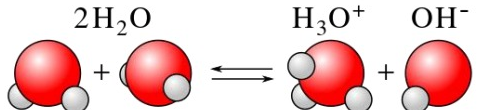
\includegraphics[width=0.45\textwidth]{images_crop_hoa11_de01/cau4_mo_hinh_nuoc.png}
\end{center}
\choiceTF
{a) Hai phân tử nước trong phương trình điện li trên là acid.}
{b) Hai phân tử nước trong phương trình điện li trên là base.}
{\True c) Nước là một chất lưỡng tính vì nó có thể đóng vai trò là một acid hoặc một base.}
{\True d) Hai phân tử nước trong phương trình điện li trên một phân tử đóng vai trò acid và một phân tử đóng vai trò base.}
\loigiai{
Trong phương trình $2\ce{H2O <=> H3O+ + OH-}$:\\
- Một phân tử $\ce{H2O}$ nhường proton $\ce{H+}$ đóng vai trò là acid.\\
- Phân tử $\ce{H2O}$ kia nhận proton $\ce{H+}$ đóng vai trò là base.\\
➔ Do đó nước là chất lưỡng tính theo Brønsted – Lowry. Ý a, b sai; ý c, d đúng.}
\end{ex}

\bigskip
\noindent
\textbf{PHẦN III (1,5 điểm -- 6 câu): Câu trắc nghiệm yêu cầu trả lời ngắn.}\\
\textit{Thí sinh trả lời từ câu 1 đến câu 6.}

\begin{ex}
Nồng độ mol của ion $\ce{NO3-}$ trong dung dịch $\ce{Ba(NO3)2}\ 0{,}1\text{ M}$ là x M. Xác định giá trị của x.
\shortans{0{,}2}
\loigiai{
$\ce{Ba(NO3)2 -> Ba^{2+} + 2NO3-}$\\
$0{,}1\text{ M} \longrightarrow \quad\quad\ 0{,}2\text{ M}$\\
Vậy $[\ce{NO3-}] = 0{,}2\text{ M} \implies x = 0{,}2$.\\
\textbf{Đáp án: 0,2.}}
\end{ex}

\begin{ex}
(SBT-CTST): Để chuẩn độ 40 mL dung dịch $\ce{HCl}$ chưa biết nồng độ đã dùng trung bình hết 34 mL dung dịch $\ce{NaOH}\ 0{,}12\text{ M}$. Tính nồng độ mol của dung dịch $\ce{HCl}$.
\shortans{0{,}102}
\loigiai{
$n_{\ce{NaOH}} = 0{,}034 \times 0{,}12 = 0{,}00408\text{ mol}$.\\
$\ce{HCl + NaOH -> NaCl + H2O} \implies n_{\ce{HCl}} = n_{\ce{NaOH}} = 0{,}00408\text{ mol}$.\\
$C_{M(\ce{HCl})} = \frac{0{,}00408}{0{,}040} = 0{,}102\text{ M}$.\\
\textbf{Đáp án: 0,102.}}
\end{ex}

\begin{ex}
{[CD - SBT]} Xác định pH của dung dịch thu được sau khi thêm 25,0 ml dung dịch $\ce{NaOH}\ 0{,}1\text{M}$ vào 50,0 ml dung dịch $\ce{HCl}\ 0{,}1\text{ M}$.
\shortans{1{,}48}
\loigiai{
$n_{\ce{NaOH}} = 0{,}025 \times 0{,}1 = 2{,}5 \cdot 10^{-3}\text{ mol}$; $n_{\ce{HCl}} = 0{,}050 \times 0{,}1 = 5{,}0 \cdot 10^{-3}\text{ mol}$.\\
$\ce{H+ + OH- -> H2O} \implies n_{\ce{H+ dư}} = 5{,}0 \cdot 10^{-3} - 2{,}5 \cdot 10^{-3} = 2{,}5 \cdot 10^{-3}\text{ mol}$.\\
$V_{\text{dd}} = 25{,}0 + 50{,}0 = 75{,}0\text{ mL} = 0{,}075\text{ L}$.\\
$[\ce{H+}] = \frac{2{,}5 \cdot 10^{-3}}{0{,}075} \approx 0{,}0333\text{ M} \implies \text{pH} = -\log(0{,}0333) \approx 1{,}48$.\\
\textbf{Đáp án: 1,48.}}
\end{ex}

\begin{ex}
{[CD - SBT]} Có bao nhiêu phát biểu nào dưới đây là đúng trong số các phát biểu đã cho dưới đây?\\
(a) Để so sánh mức độ acid giữa các dung dịch có thể dựa vào nồng độ: dung dịch acid nào có nồng độ lớn hơn sẽ có tính acid mạnh hơn.\\
(b) Trong các dung dịch có cùng nồng độ, dung dịch nào có tính acid mạnh hơn sẽ có nồng độ ion $\ce{H+}$ lớn hơn và pH lớn hơn.\\
(c) Trong các dung dịch có cùng nồng độ, dung dịch nào có nồng độ ion $\ce{OH-}$ lớn hơn và pH nhỏ hơn sẽ có tính base lớn hơn.\\
(d) Trong các dung dịch có cùng nồng độ, dung dịch nào có tính acid mạnh hơn sẽ có nồng độ ion $\ce{H+}$ lớn hơn và pH nhỏ hơn.\\
(e) Trong các dung dịch có cùng nồng độ, dung dịch có nồng độ ion $\ce{H+}$ nhỏ hơn và pH cao sẽ có tính acid yếu hơn.\\
(g) Trong một dãy các dung dịch có cùng nồng độ được sắp xếp theo tính acid tăng dần thì nồng độ ion $\ce{OH-}$ sẽ giảm dần và $K_a$ tăng dần.
\shortans{3}
\loigiai{
Có 3 phát biểu đúng là: (d), (e), (g).\\
- (a) Sai vì độ mạnh acid phụ thuộc vào khả năng phân li ra $\ce{H+}$.\\
- (b) Sai vì tính acid mạnh hơn thì pH phải nhỏ hơn.\\
- (c) Sai vì tính base lớn hơn thì pH phải lớn hơn.\\
- (d) Đúng vì acid càng mạnh thì $[\ce{H+}]$ càng lớn và pH càng nhỏ.\\
- (e) Đúng vì $[\ce{H+}]$ càng nhỏ (pH càng cao) thì tính acid càng yếu.\\
- (g) Đúng vì tính acid tăng dần thì $[\ce{OH-}]$ giảm dần và $K_a$ tăng dần.\\
\textbf{Đáp án: 3.}}
\end{ex}

\begin{ex}
{[CD - SGK]} Để trung hoà 10mL dung dịch $\ce{HCl}$ nồng độ x M cần 50 ml dung dịch $\ce{NaOH}\ 0{,}5\text{ M}$. Xác định giá trị của x.
\shortans{2{,}5}
\loigiai{
$n_{\ce{NaOH}} = 0{,}050 \times 0{,}5 = 0{,}025\text{ mol}$.\\
$\ce{HCl + NaOH -> NaCl + H2O} \implies n_{\ce{HCl}} = n_{\ce{NaOH}} = 0{,}025\text{ mol}$.\\
$x = C_{M(\ce{HCl})} = \frac{0{,}025}{0{,}010} = 2{,}5\text{ M}$.\\
\textbf{Đáp án: 2,5.}}
\end{ex}

\begin{ex}
(SBT - KNTT): Vỏ trứng có chứa calcium ở dạng $\ce{CaCO3}$. Để xác định hàm lượng $\ce{CaCO3}$ trong vỏ trứng, trong phòng thí nghiệm người ta có thể làm như sau:\\
Lấy 1,0 g vỏ trứng khô, đã được làm sạch, hoà tan hoàn toàn trong 50 mL dung dịch $\ce{HCl}\ 0{,}4\text{ M}$. Lọc dung dịch sau phản ứng thu được 50 mL dung dịch A. Lấy 10,0 mL dung dịch A chuẩn độ với dung dịch $\ce{NaOH}\ 0{,}1\text{ M}$ thấy hết 5,6 mL. Xác định hàm lượng $\ce{CaCO3}$ trong vỏ trứng (giả thiết các tạp chất khác trong vỏ trứng không phản ứng với $\ce{HCl}$). Kết quả làm tròn đến hàng đơn vị phần trăm.
\shortans{86\%}
\loigiai{
- Ban đầu trong 50 mL $\ce{HCl}\ 0{,}4\text{ M}$: $n_{\ce{HCl ban đầu}} = 0{,}050 \times 0{,}4 = 0{,}02\text{ mol}$.\\
- Chuẩn độ 10,0 mL A: $n_{\ce{NaOH}} = 0{,}0056 \times 0{,}1 = 5{,}6 \cdot 10^{-4}\text{ mol} \implies n_{\ce{HCl (10 mL A)}} = 5{,}6 \cdot 10^{-4}\text{ mol}$.\\
- Trong 50 mL A (lượng $\ce{HCl}$ dư): $n_{\ce{HCl dư}} = 5{,}6 \cdot 10^{-4} \times \frac{50}{10} = 2{,}8 \cdot 10^{-3}\text{ mol}$.\\
- Lượng $\ce{HCl}$ đã phản ứng: $n_{\ce{HCl pứ}} = 0{,}02 - 0{,}0028 = 0{,}0172\text{ mol}$.\\
- Phản ứng: $\ce{CaCO3 + 2HCl -> CaCl2 + CO2 + H2O}$\\
$\implies n_{\ce{CaCO3}} = \frac{1}{2} n_{\ce{HCl pứ}} = \frac{0{,}0172}{2} = 8{,}6 \cdot 10^{-3}\text{ mol}$.\\
- Khối lượng $\ce{CaCO3}$: $m = 8{,}6 \cdot 10^{-3} \times 100 = 0{,}86\text{ g}$.\\
- Hàm lượng: $\%m_{\ce{CaCO3}} = \frac{0{,}86}{1{,}0} \times 100\% = 86\%$.\\
\textbf{Đáp án: 86\%.}}
\end{ex}

\bigskip
\noindent
\textbf{PHẦN IV: Tự luận}\\
\textit{Học sinh giải chi tiết các bài toán sau vào giấy làm bài.}

\begin{ex}
{[CD - SBT]} Điền từ ngữ thích hợp vào các chỗ trống trong mỗi phát biểu sau:
\begin{enumerate}[a)]
	\item Phản ứng thuận nghịch là phản ứng hóa học trong đó ở cùng điều kiện, xảy ra ...(1)... sự chuyển chất phản ứng thành sản phẩm và sự chuyển ...(2)... thành ...(3)...
	\item Trạng thái cân bằng của mọi phản ứng thuận nghịch luôn có tốc độ phản ứng thuận ...(1)... tốc độ phản ứng nghịch, các phản ứng thuận và nghịch luôn diễn ra. Như vậy, cân bằng hóa học là ...(2)...
	\item Với một phản ứng hóa học, khi hằng số cân bằng rất lớn so với 1 thì ở trạng thái cân bằng, nồng độ các chất sản phẩm ...(1)... nồng độ ...(2)...
\end{enumerate}
\loigiai{
a) (1) đồng thời; (2) chất sản phẩm; (3) chất phản ứng.\\
b) (1) bằng; (2) cân bằng động.\\
c) (1) lớn hơn; (2) các chất phản ứng.}
\end{ex}

\begin{ex}
{[CTST - SGK]} Ở các vùng quê, người dân thường dùng phèn chua để làm trong nước nhờ ứng dụng của phản ứng thuỷ phân ion $\ce{Al^3+}$? Giải thích? Chất hay ion nào là acid, là base trong phản ứng thuỷ phân $\ce{Al^3+}$?
\begin{center}
	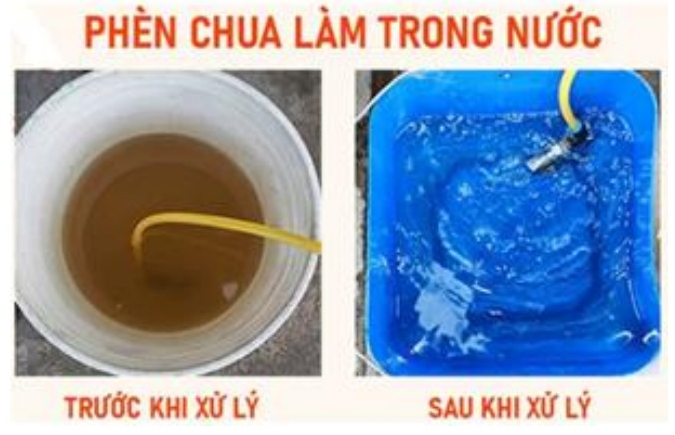
\includegraphics[width=0.45\textwidth]{images_crop_hoa11_de01/cau2_tuan_phen_chua.png}
\end{center}
\loigiai{
- Khi hòa tan phèn chua ($\ce{KAl(SO4)2.12H2O}$) vào nước, ion $\ce{Al^3+}$ bị thuỷ phân tạo thành phức $[\ce{Al(H2O)6}]^{3+}$. Ion này nhường proton $\ce{H+}$ cho nước theo cân bằng:\\
\[ [\ce{Al(H2O)6}]^{3+} + \ce{H2O <=> [Al(OH)(H2O)5]^{2+} + H3O+} \]
hoặc viết gọn: $\ce{Al^3+ + 3H2O <=> Al(OH)3 v + 3H+}$.\\
- Kết tủa $\ce{Al(OH)3}$ dạng keo xốp, lơ lửng trong nước, có bề mặt hấp phụ rất lớn nên sẽ kéo dính các hạt bụi bẩn lơ lửng lại và lắng nhanh xuống đáy, làm nước trở nên trong sạch.\\
- Trong phản ứng thủy phân trên: $\ce{Al^3+}$ (dạng $[\ce{Al(H2O)6}]^{3+}$) nhường $\ce{H+}$ nên là \textbf{acid}; $\ce{H2O}$ nhận $\ce{H+}$ nên đóng vai trò là \textbf{base}.}
\end{ex}

\bigskip
\noindent
{\color{hfRed}\textbf{\large BẢNG TỔNG HỢP ĐÁP ÁN ĐỀ SỐ 1}}

\smallskip
\noindent
\textbf{1. PHẦN I (Trắc nghiệm nhiều phương án):}
\begin{center}
\begin{tabular}{|c|c|c|c|c|c|c|c|c|}
\hline
\textbf{1. D} & \textbf{2. D} & \textbf{3. C} & \textbf{4. B} & \textbf{5. C} & \textbf{6. A} & \textbf{7. C} & \textbf{8. C} & \textbf{9. B} \\ \hline
\textbf{10. A} & \textbf{11. D} & \textbf{12. C} & \textbf{13. C} & \textbf{14. B} & \textbf{15. A} & \textbf{16. C} & \textbf{17. D} & \textbf{18. B-A} \\ \hline
\end{tabular}
\end{center}

\noindent
\textbf{2. PHẦN II (Trắc nghiệm đúng sai):}
\begin{itemize}
	\item \textbf{Câu 1:} a) Đúng \quad|\quad b) Sai \quad|\quad c) Sai \quad|\quad d) Đúng
	\item \textbf{Câu 2:} a) Đúng \quad|\quad b) Đúng \quad|\quad c) Đúng \quad|\quad d) Đúng
	\item \textbf{Câu 3:} a) Sai \quad|\quad b) Sai \quad|\quad c) Đúng \quad|\quad d) Đúng
	\item \textbf{Câu 4:} a) Sai \quad|\quad b) Sai \quad|\quad c) Đúng \quad|\quad d) Đúng
\end{itemize}

\noindent
\textbf{3. PHẦN III (Trả lời ngắn):}
\begin{center}
\begin{tabular}{|c|c|c|c|c|c|}
\hline
\textbf{Câu 1} & \textbf{Câu 2} & \textbf{Câu 3} & \textbf{Câu 4} & \textbf{Câu 5} & \textbf{Câu 6} \\ \hline
0,2 & 0,102 & 1,48 & 3 & 2,5 & 86\% \\ \hline
\end{tabular}
\end{center}

\begin{center}
\textbf{--------- HẾT ---------}
\end{center}

\end{document}
